\section{Platine A als Single-Tone Sender}
Für den ersten Teil des Versuchs werden zwei identische Transceiver-Platinen verwendet, die bereits im Verlauf dieses Praktikums genauer betrachtet wurden.
Die beiden Platinen haben folgende Spezifikationen:\\ 

\begin{table}[h!]
    \centering
    \begin{tabular}{|c|c|c|c|}
        \hline
         & J1 & J2 & Funktion \\
        \hline
        Platine A & \textcolor{red}{X} & \textcolor{green}{\checkmark} & Sender \\
        Platine B &\textcolor{red}{X} & \textcolor{red}{X} & Empfänger \\
        \hline
    \end{tabular}
    \caption{Spezifikationen der beiden Platinen}
    \end{table}
Die folgenden Abbildungen 4.1 und 4.2 zeigen auf der linken Seite die Platine A als Sender und auf der rechten Seite
die Platine B als Empfänger. Die äußeren Lampen am USB-Port leuchten bei Stromversorgung. Befinden sich Sender und Empfänger innerhalb der Funkreichweite, so leuchtet weder die Lampe TX (engl. transmitting: senden) noch die Lampe RX (engl. receiving: empfangen) am Sender und Empfänger.
Ist die Funkreichweite überschritten, so leuchtet die Lampe RX am Empfänger, die Lampe TX leuchtet nicht. Der Sender bleibt unverändert. 
\begin{figure}[H]
    \centering
    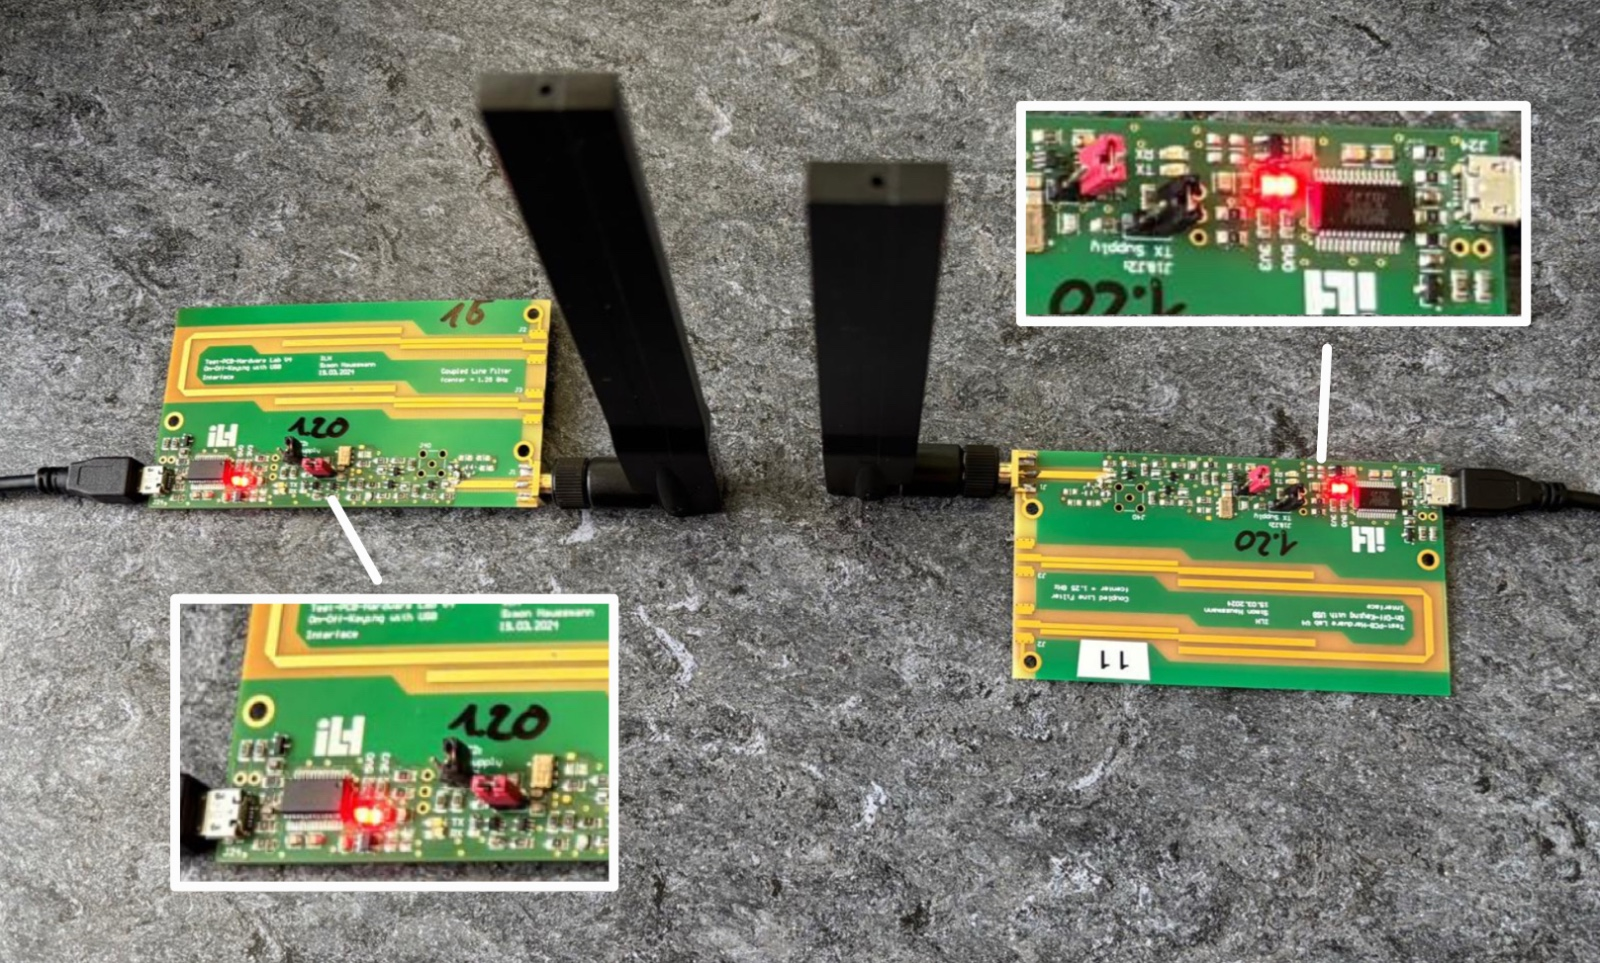
\includegraphics[width=0.8\textwidth]{Pictures/Task2aa.jpg}
    \caption{Sender und Empfänger innerhalb der Funkreichweite}
    \label{fig:Task2aa}
\end{figure}

\begin{figure}[H]
    \centering
    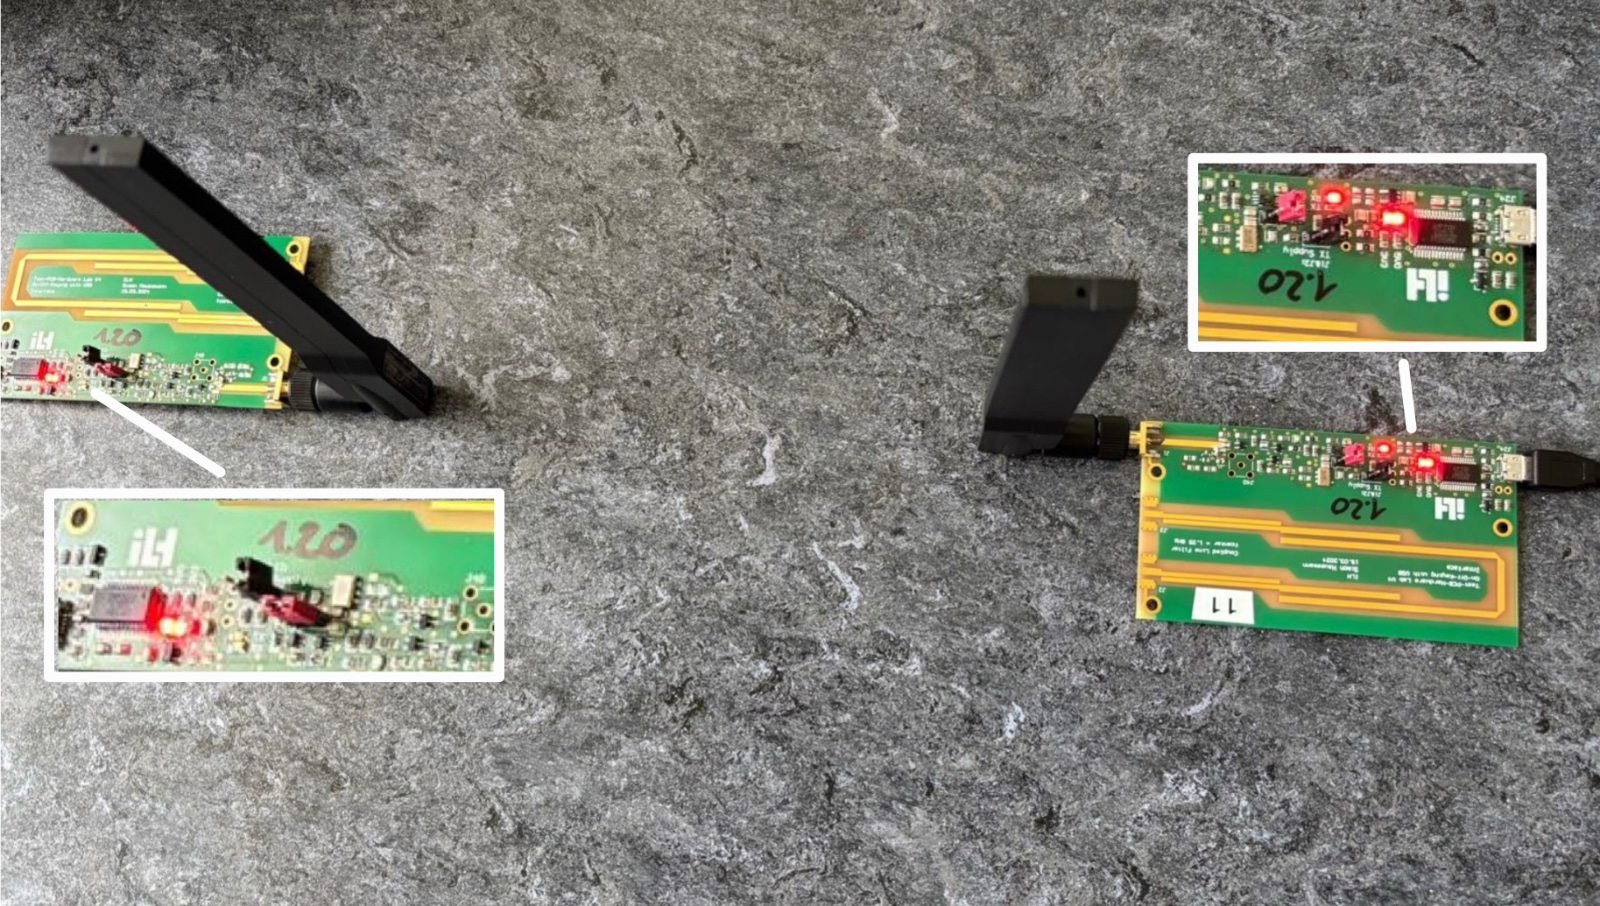
\includegraphics[width=0.8\textwidth]{Pictures/Task2a.jpg}
    \caption{Sender und Empfänger außerhalb der Funkreichweite}
    \label{fig:Task2a}
\end{figure}
Nun betrachten wir die Funkreichweite der Platinen genauer. Diese Messung führen wir auf zwei unterschiedliche
Arten durch. Einmal wird der Abstand der beiden Antennen innerhalb der Funkreichweite erhöht, bis der Kontakt
abbricht. Dann wird der Abstand der Antennen außerhalb der Funkreichweite verringert, bis der Kontakt wieder
hergestellt ist. Zuerst wurde eine Funkreichweite von $d_{TR,1}=9\,\text{cm}$ gemessen. Auf die zweite Art wurde eine
Funkreichweite von $d_{TR,2}=8\,\text{cm}$ gemessen. Dies kann auf das Schwellverhalten des Empfängers (Hysterese-Effekt)
zurückzuführen sein. 
Ein schwaches Signal kann noch von der Platine B empfangen werden, wobei die Verbindung unzureichend ist, um 
initial erkannt zu werden.\\
Die maximale Funkreichweite der Platinen, um Signale sicher auszuwerten, beträgt somit $d_{TR,max}=8\,\text{cm}$.
\\
Nun wird der Versuch wiederholt, jedoch wird die Funktion der Platinen getauscht. Wie zu erwarten, ist das Ergebnis
im Rahmen der Messungenauigkeit identisch. Die Funkreichweite beträgt ebenfalls $d_{TR,1}=9\,\text{cm}$ und $d_{TR,2}=8\,\text{cm}$ und 
hat somit ebenfalls eine maximale Funkreichweite der Platinen, um sicher Signale auszuwerten, von $d_{TR,max}=8\,\text{cm}$.

\section{Platinen am Computer anschließen}
Nun wurde eine Platine an den Computer angeschlossen und die andere Platine an den Laptop.
Mithilfe von Hterm werden Daten in Form von ASCII-Zeichen von der einen Platine an die andere gesendet
und mit Hterm wieder ausgelesen.
Wichtig in dieser Prozedur war das Verbinden beider Jumper an der Sender-Platine und das Entfernen beider
Jumper an der Empfänger-Platine. 
Wären die Jumper bei der Empfänger-Platine verbunden gewesen, wäre das Problem gewesen, dass die Platine auch 
ein Signal gesendet hätte und dieses auch wieder empfangen hätte, was unerwünscht ist.
In der Praxis konnten wir mit diesem Setup eine nutzbare Reichweite von etwa 7,5\,cm erreichen.

\begin{table}[h!]
    \centering
    \begin{tabular}{|c|c|c|c|}
        \hline
         & J1 & J2 & Funktion \\
        \hline
        Platine A & \textcolor{green}{\checkmark} & \textcolor{green}{\checkmark} & Sender \\
        Platine B &\textcolor{red}{X} & \textcolor{red}{X} & Empfänger \\
        \hline
    \end{tabular}
    \caption{Spezifikationen der beiden Platinen}
\end{table}

\section{BER-Messung}
Jetzt wird das zur Verfügung gestellte
Matlab-Skript \texttt{BER\_Measurement.m} genutzt, um eine Bit-Error-Analyse der Verbindung durchzuführen.
Zuerst werden die Platinen so ausgerichtet, dass sich die Antennen parallel zueinander befinden und sich berühren.
Aus dieser Position heraus wird die Übertragungsstrecke schrittweise in 1-cm-Schritten inkrementiert und die BER dokumentiert.


\begin{table}[h!]
    \centering
        \begin{tabular}{c|c}
            Abstand [cm] & BER A $\rightarrow$ B \\
            \hline
             0 & 0.00 \\
            \hline
             1 & 0.00 \\
            \hline
             2 & 0.64 \\
            \hline
             3 &  1.00 \\
            \hline
             4 &   1.00 \\
            \hline
             5 & 1.00 \\
            \hline
             6 & 1.00 \\
        \end{tabular}
        \caption{Übertragung mit Platine A als Sender und Platine B als Empfänger}
    \end{table}
In der Messreihe Tabelle 4.3 wurde die Platine A als Sender und Platine B als Empfänger konfiguriert.
Es ist zu erkennen, dass die BER für einen Abstand von 0–1\,cm null ist. Im nächsten Zentimeter
steigt sie auf 0,64 an und ist bereits 1\,cm später auf 1,00 angestiegen. Das bedeutet eine
hundertprozentige Fehlerbitrate.\\

Nun wurde die Funktion der Platinen getauscht, sodass Platine B als Sender und Platine A als Empfänger fungiert. Die Ergebnisse
sind in Tabelle 4.4 zu sehen.
\begin{table}[h!]
    \centering
        \begin{tabular}{c|c}
            Abstand [cm] & BER B $\rightarrow$ A \\
            \hline
             0 & 0.00 \\
            \hline
             1 & 0.00 \\
            \hline
             2 & 0.00 \\
            \hline
             3 & 0.00 \\
            \hline
             4 & 0.03 \\
            \hline
             5 & 1.00 \\
            \hline
             6 & 1.00 \\
        \end{tabular}
        \caption{Übertragung mit Platine B als Sender und Platine A als Empfänger}
    \end{table}
    \\
    
Hier ist der Bitfehler bis zu einem Abstand von 3\,cm null. Er steigt bei 4\,cm auf 0,03 an und ist
danach auf hundert Prozent angestiegen.\\
Zum besseren Vergleich sind die Messwerte zusätzlich in Abbildung 4.3 grafisch dargestellt.

\begin{figure}[H]
    \centering
    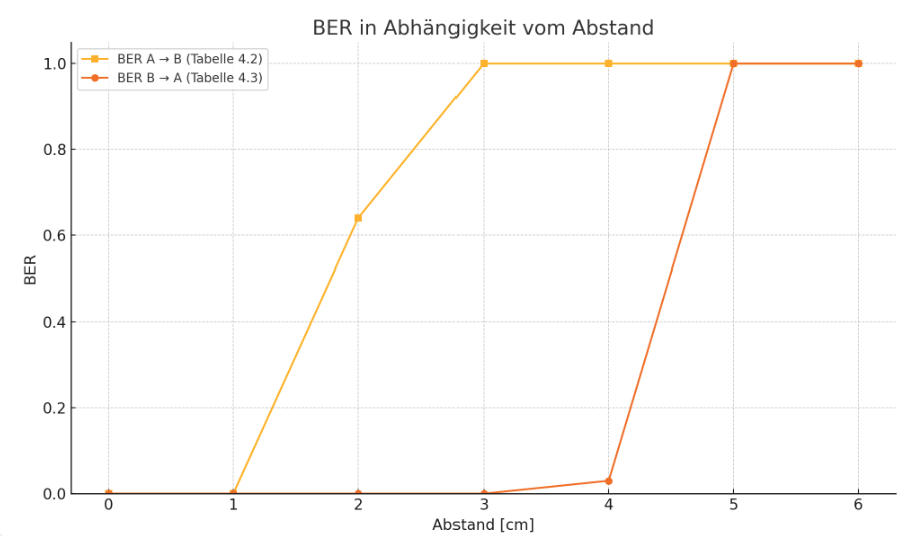
\includegraphics[width=0.8\textwidth]{Pictures/diagramm.png}
    \caption{Vergleich BER-Messung der Platinen}
\end{figure}

Der BER von der Empfänger- zur Senderplatine wird ebenfalls aufgezeichnet. Dieser ist jedoch
immer ein hundertprozentiger Fehler.
Man kann erkennen, dass beide Platinen alles andere als optimal für die Datenübertragung sind und
dass sie auch untereinander erhebliche Unterschiede aufweisen. Die Konfiguration mit Platine B als Sender und A als Empfänger erreicht jedoch
das bestmögliche Ergebnis.


\section{Interessante/Witzige Beobachtung}
Als wir die Messung von Task 4 durchgeführt haben und dann bei größeren Entfernungen kein Signal mehr erfasst hatten,
haben wir aus Spaß einen Samsung-Pen auf beide Antennen gelegt und auf einmal konnten wir wieder Signale empfangen.
Ein möglicher Grund dafür könnte sein, dass der Samsung-Pen metallische Bestandteile enthält,
die die EM-Welle besser leiten als Luft.

\begin{figure}[H]
    \centering
    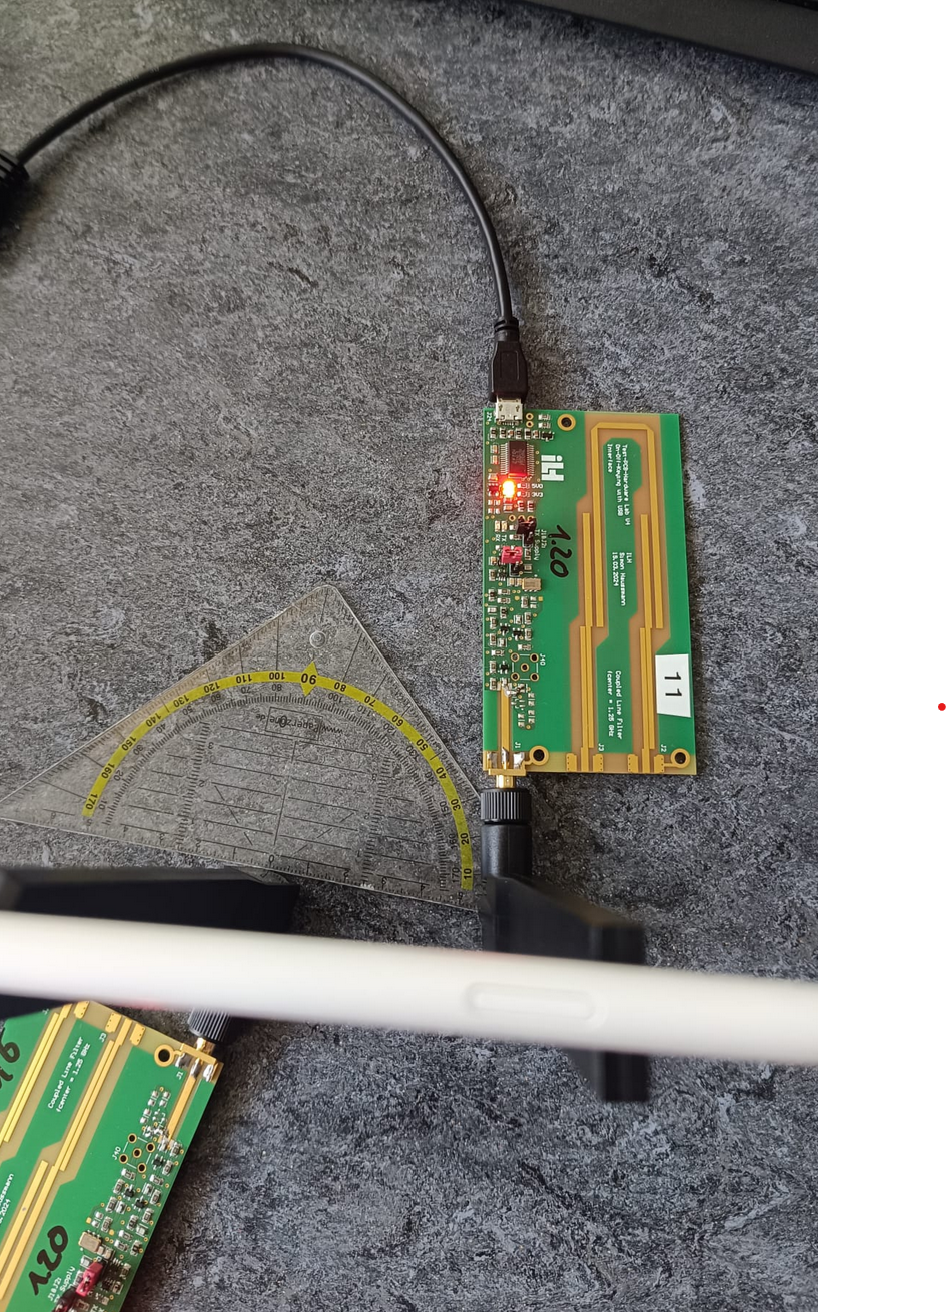
\includegraphics[width=0.4\textwidth]{Pictures/stift.png}
    \caption{Samsung Pen auf Antenne}
\end{figure}

\clearpage

\section{Bildübertragung über Funkverbindung}
Zu guter Letzt wird eine Bildübertragung über eine sehr kurze Funkstrecke durchgeführt. Das folgende Originalbild wird hierbei übertragen:
\begin{figure}[H]
    \centering
    
\includegraphics[width=0.6\textwidth]{Pictures/meme.jpg}
    \caption{Das zu übertragende Originalbild}
    \label{fig:Task2b}
\end{figure}

Unser Verwendetes Bild hat das Format .png. Dessen ASCII Zeichen ansammlung wird wie zuvor nacheinander übertragen.
\subsection{Übertragung bei sehr kurzer Funkstrecke}
Ein Ausschnitt aus der Sammlung der ASCII-Zeichen, die übertragen wurden, ist in Abbildung \ref{fig:Task2c} zu sehen.

\begin{figure}[H]
    \centering
    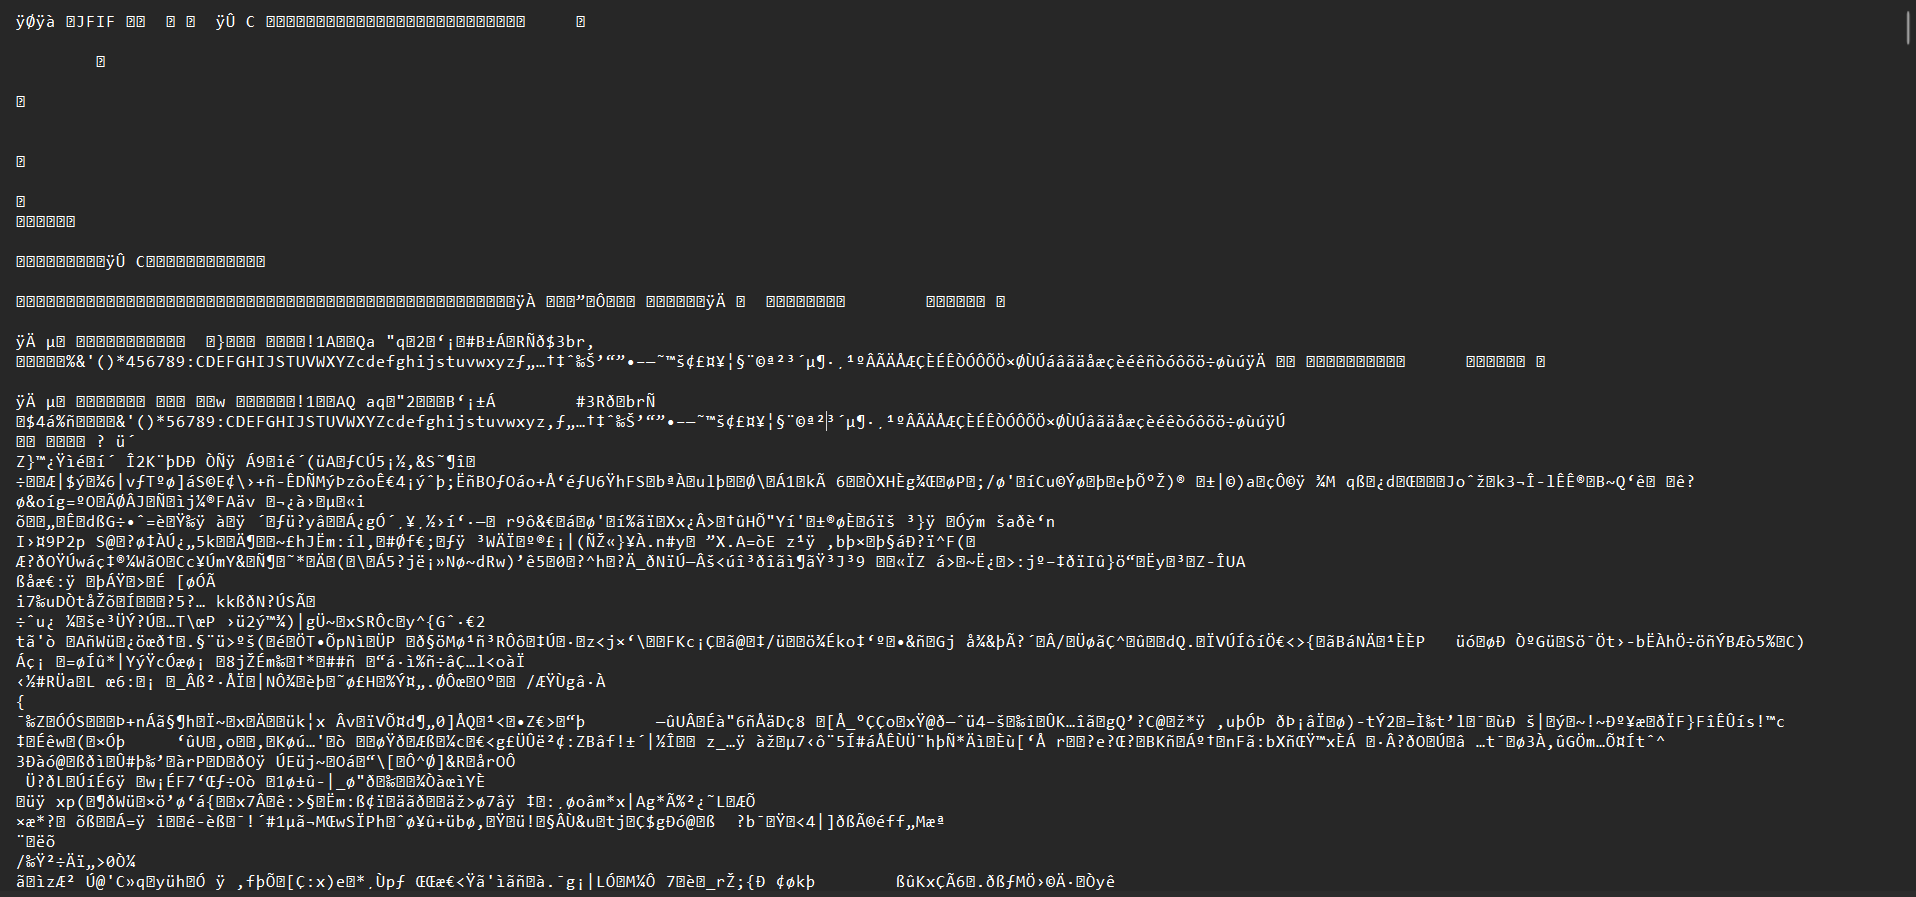
\includegraphics[width=0.8\textwidth]{Pictures/memeASCII.png}
    \caption{Das übertragene Bild in ASCII-Darstellung}
    \label{fig:Task2c}
\end{figure}

In dem Format ist die Datei für den Menschen nicht lesbar, da sie aus einer Vielzahl von Zeichen besteht, die nicht direkt interpretiert werden können. 
Die Änderung der Dateierweiterung in .png stellt sicher, dass das Bild tatsächlich als ein Bild dargestellt wird. 

Die Datei lässt sich hierbei bei einer sehr kurzen Funkstrecke problemlos öffnen, was davon überzeugt, dass die Fehlerbitrate bei einer geringen bzw. gar nicht vorhandenen Distanz zwischen Sender und Empfänger sehr gering ist.

\subsection{Übertragung bei größerer Funkstrecke}
Wird jetzt aber eine längere Funkstrecke zwischen Sender und Empfänger gewählt, so ändert sich das Verhalten der Übertragung. 

Es stellte sich in der Praxis heraus, dass die Übertragungsqualität bei einer größeren Funkstrecke deutlich abnimmt.

In Abbildung \ref{fig:Task2d} sind die Bilder zu sehen, die mit kleiner werdender Funkstrecke übertragen wurden.
\begin{figure}[H]
    \begin{minipage}{0.45\textwidth}
            \centering
            
\includegraphics[width=\linewidth]{Pictures/grosserAbstand.jpg}
        \end{minipage}
        \hfill
        \begin{minipage}{0.45\textwidth}
            \centering
            
\includegraphics[width=\linewidth]{Pictures/wenigergrosserabstand.jpg}
        \end{minipage}

        \vspace{0.5cm}

        \begin{minipage}{0.45\textwidth}
            \centering
            
\includegraphics[width=\linewidth]{Pictures/nochwenigergrosserabstand.jpg}
        \end{minipage}
        \hfill
        \begin{minipage}{0.45\textwidth}
            \centering
            
\includegraphics[width=\linewidth]{Pictures/kleinerabstand.jpg}  
        \end{minipage}   
    \caption{Das übertragene Bild bei verschiedenen Funkstrecken}
    \label{fig:Task2d} 
    \end{figure}


Man sieht deutlich, dass die Übertragung bei größerer Funkstrecke zu Störungen führt, die sich in Form von fehlenden Pixeln im Bild äußern. 
In der Praxis war die Änderung des Abstands im Bild 4 relativ zu Bild 3 vergleichsweise klein, hatte jedoch eine massive Verbesserung der Übertragungsqualität zur Folge.
\\
Da auf den oberen Bildern bei weiterer Entfernung fast nix mehr zu sehen ist, selbst nach mehrfachen Wiederholungen.
Haben wir während die Platine gesendet hat, kurz die Entfernung erhöht und wieder verringert. Das Ergebnis der Bildübertragung ist dann das folgende:
\begin{figure}[H]
    \centering
    
\includegraphics[width=0.6\textwidth]{Pictures/memeASCIIbewegt.jpg}
    \caption{Das übertragene Bild in ASCII bei bewegten Platinen}
    \label{fig:Task2e}
\end{figure}
%Bei der oberen Darstellung ist zu beachten, dass aufgrund der LaTeX-Formatierung das Bild im unteren Teil, das nicht korrekt übertragen wurde, schwarz gefärbt ist. Der untere Teil müsste aber weiß sein, da ein nicht übertragendes Zeichen null ist und null steht für weiß.
\subsection{Abhilfemaßnahmen zur Verbesserung trotz Bitfehler}
Eine Möglichkeit zur besseren Signalübertragung wäre MIMO (Multiple Input Multiple Output). MIMO nutzt mehrere Antennen zur Datenübertragung und -empfang. Dadurch wird eine erhöhte Diversität des Signals und somit eine höhere Robustheit gegenüber Fehlern erreicht.\footnote{Vgl. Wikipedia. Online:\url{https://de.wikipedia.org/wiki/MIMO_(Nachrichtentechnik)} (abgerufen am 08.07.2025).}

Die zweite Möglichkeit wäre es, dieselbe Information mehrfach zu senden (zeitlich oder räumlich). Der Empfänger kombiniert die Signale und stellt somit eine robuste Decodierung sicher.\footnote{Vgl. Diversity scheme. In: Wikipedia. Online:\url{https://en.wikipedia.org/wiki/Diversity_scheme?utm_source=chatgpt.com} (abgerufen am 08.07.2025)}
